\documentclass[a4paper,12pt,authoryear]{elegantpaper}
    \usepackage[ruled,linesnumbered]{algorithm2e}
    \usepackage{hyperref}
    \title{Report of Matrix Completion in Frontier Literature Selection I}
    \author{Ziyang Gong \thanks{Email: \email{meetziyang@outlook.com}}}
    \institute{School of Statistics, Southwest University of Finance and Economics}
    \date{}

\begin{document}

    \maketitle

    There has been an increasing awareness of missing data in statistical practice. The problem exists but is not welcome since the incomplete dataset cannot directly apply most statistical methods. One of the critical approaches to deal with missing data is imputing missing values by plausible values. Therefore, the imputed dataset can directly apply any statistical method. This problem has also been known as matrix completion, i.e., imputing missing values by plausible values with the matrix form.

    There has been a wide range of applications in practice life. For instance, one may have a matrix of customers and products, with entries recording the number of purchases. There will typically be a high proportion of missing entries. We aim to identify items that distinguish customers' preferences incredibly effectively, make recommendations to users of products they might like, and efficiently summarize customers' preferences. This question can also be solved by matrix completion method.

    If there are no other assumptions, there is no way to solve the matrix completion problem. To solve this problem, we usually implicitly assume that \textbf{the real matrix is low-rank}. So matrix completion can be transformed into the following optimization problem:
    \begin{equation}
        \label{equation:standard_matrix_completion}
        \begin{array}{ll}
        \min _{\bf X} & \operatorname{rank}(\bf X) \\
        \text { s.t. } & P_{\bf\Omega}(\bf X)=P_{\bf\Omega}(\bf M)
        \end{array}
    \end{equation}
    where $\bf X$ is the estimated matrix, $\bf M$ is the observed matrix, $\bf\Omega$ is the index of observed entries, projection operator $P_{\bf\Omega}(\bf X)$ is
    \begin{equation*}
        \left|P_{\bf\Omega}(\bf X)\right|_{i, j}=\left\{\begin{array}{ll}
            \bf{X}_{i, j} & (i, j) \in \Omega \\
            0 & \text { otherwise }
            \end{array}\right.
    \end{equation*}
    Moreover, most approaches are solving the problem in this form.

    In this course, we have read three papers about matrix completion, as shown below:
    \begin{itemize}
        \item A principal components method to impute missing values for mixed data \citep{audigier_principal_2013}.
        \item Optimal adaptive matrix completion \citep{ramazanli_optimal_2020}.
        \item High-dimensional principal component analysis with heterogeneous missingness \citep{zhu_high-dimensional_2019}.
    \end{itemize}
    which discuss matrix completion from three different perspectives: type of data, the proportion of observations, and missing mechanism. In the following sections, we will review the literature on type of data and missing mechanism, summarize the methods and conclusions mentioned in the above papers, and use these approaches to analyze the real data.

    \section{Type of Data}

    Not all methods can be used for continuous data and categorical data at the same time. We usually design different models to fill different types of data.

    Several imputation approaches are available for continuous data. 
    It can be solved by factorial analysis, such as PCA methods.
    \citet{kiers_weighted_1997} proposed the PCA method, which performs PCA despite the missingness of some data, and uses the principal components and axes obtained by PCA algorithm to reconstuct the data, which provides an imputation of the missing entries.
    This method has the particular advantage of simultaneously imputing any missing data by taking into account the similarities between individuals and the relationships between variables.
    The imputation of categorical data can also be done with non-parametric methods such as the KNN method by imputing missing entries by mode of those non-missing entries of its neighbors \citep{troyanskaya_missing_2001}.

    As for mixed data, i.e., both continuous and categorical are existing. 
    \citet{stekhoven_missforest--non-parametric_2012} build a Random Forest model by setting a particular target variable with the most number of non-missing entries as the outcome and other variables as predictors, then to predict the target variable with missing entries iteratively until the prediction stabilizes. This approach is the most popular among the existing methods for several reasons: good quality of imputation whatever the number of individuals and variables, regardless of the type of relationship between variables, and it is little sensitive to the tuning parameters.

    \subsection{The Iterative FAMD Algorithm}

    As for \textit{A principal components method to impute missing values for mixed data} \citet{audigier_principal_2013} proposed the \textbf{iterative FAMD algorithm} which based on principal components method --- the factorial analysis for mixed data (FAMD) and balances the influence of all the variables that are continuous and categorical in the construction of the dimensions of variability. For convenience, the Iterative FAMD Algorithm is given in Algorithm \ref{algorithm:iterative_famd}. 

    \begin{figure}[!hbt]
        \centering
        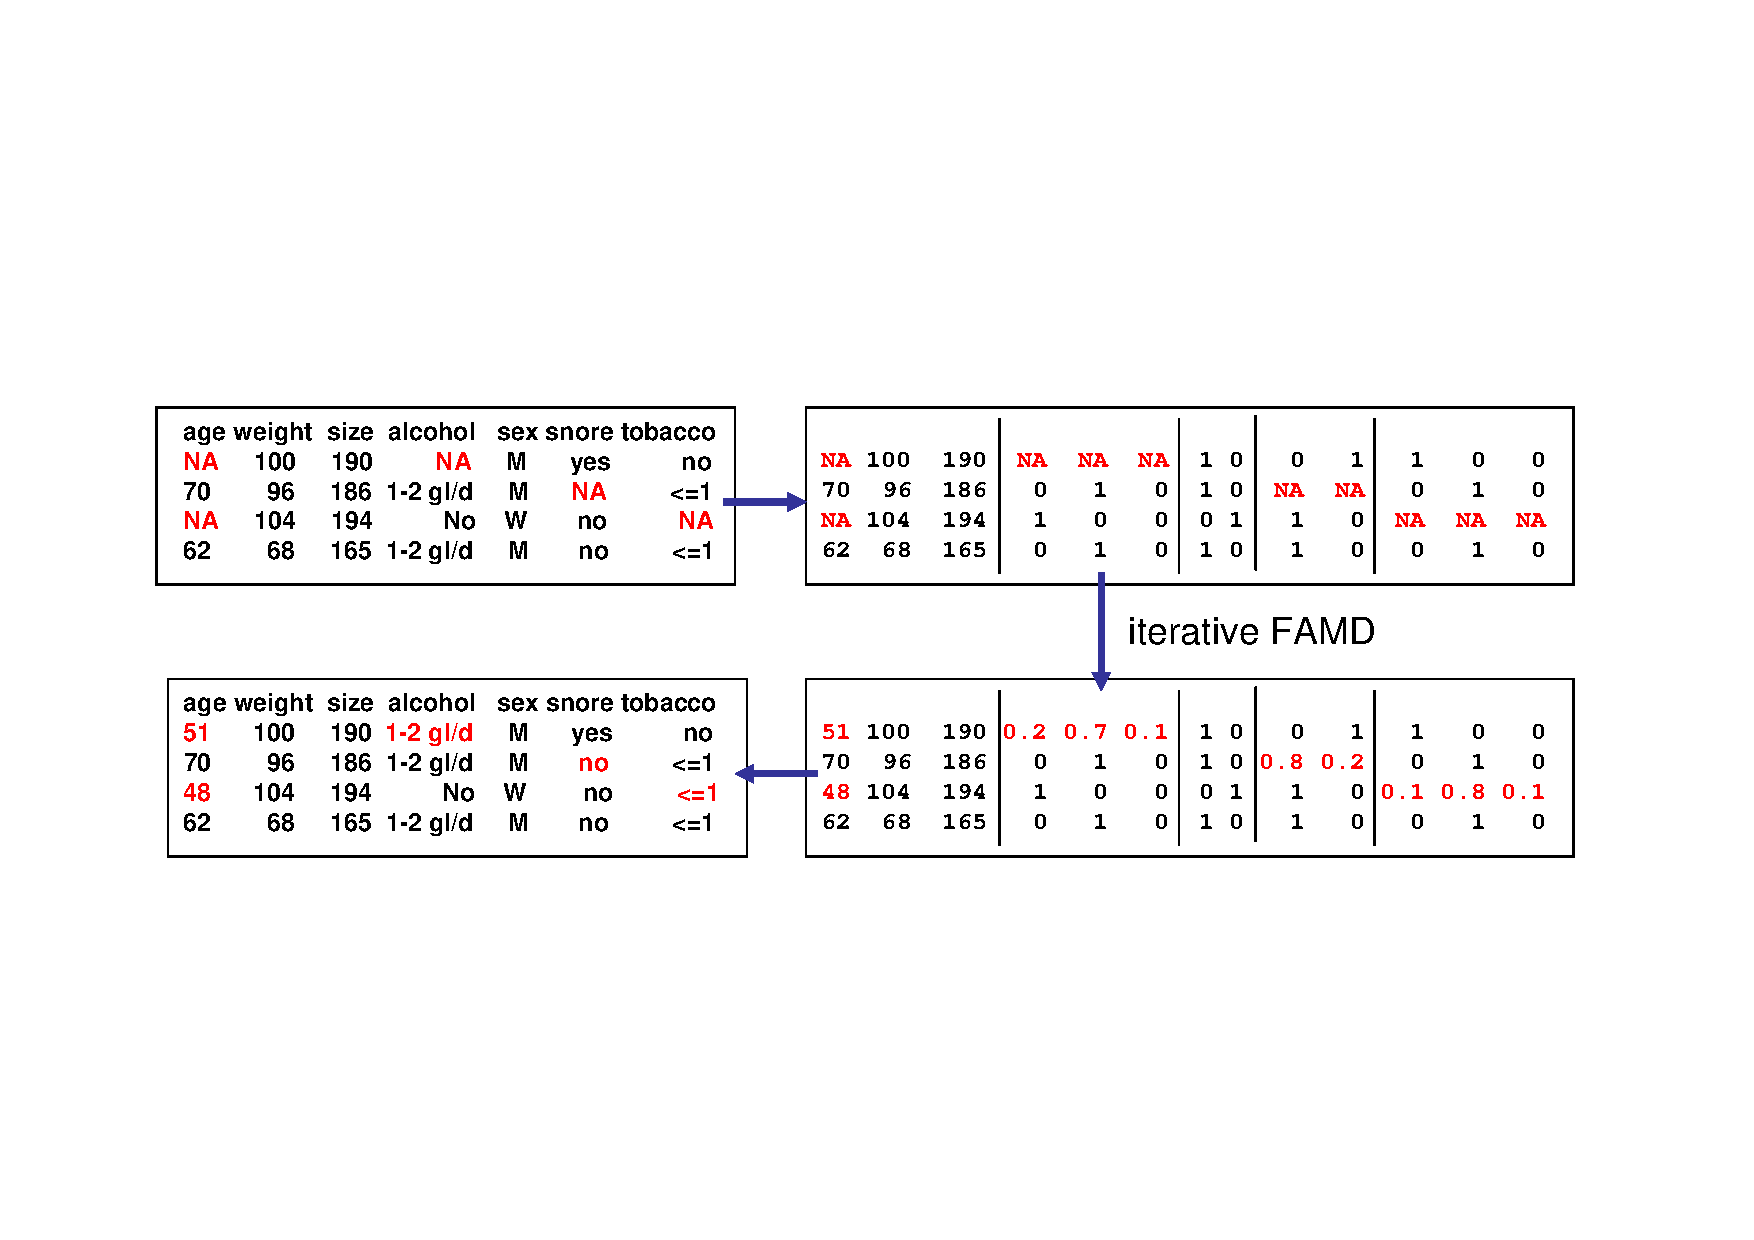
\includegraphics[width=0.9\textwidth]{./figures/algo_afdm.pdf}
        \caption{Diagram for the iterative FAMD algorithm: the raw mixed data, the matrix $\bf X$, the imputed data obtained by iterative FAMD and the imputed mixed data. \citep{audigier_principal_2013}}
    \end{figure}

    
    \begin{algorithm}[H]
        \KwData{observed matrix $\bf M\in\mathbb{R}^{m\times d}$, svd's rank $s$}
        \KwResult{imputed matrix $\hat{\bf M}\in\mathbb{R}^{m\times d}$}
        $\bf X\in\mathbb{R}^{m\times n}\leftarrow$ convert categorical variable in $\bf M$ into dummy variables\;
        Initialization $\ell=1$, $\bf X^{0}$, $\bf D_{\Sigma}^{0}$, $\bf M^{0}$\;
        \While{$\sum_{ij}(\hat x_{ij}^{\ell-1}-\hat x_{ij}^{\ell})^2\leq \varepsilon$}{
            $\bf C^{\ell}\leftarrow\bf X^{\ell -1}\left(\bf D_{\Sigma}^{\ell -1}\right)^{-1/2}-\bf M^{\ell-1}$\;
            $\bf C^{\ell}\leftarrow\hat{\bf U}^{\ell}\hat{\bf\Lambda}^{\ell}\left(\hat{\bf V}^{\ell}\right)^T$ be the SVD of $\bf C^{\ell}$ where $\hat{\bf U}^{\ell}\in\mathbb{R}^{m\times s}$,  $\hat{\bf V}^{\ell}\in\mathbb{R}^{s\times n}$ have orthonormal columns, $\hat{\bf\Lambda}^{\ell}\in\mathbb{R}^{s\times s}$ is diagonal\;
            $\hat{\bf X}^{\ell}\leftarrow\left(\hat{\bf U}^{\ell}\hat{\bf\Lambda}^{\ell}\left(\hat{\bf V}^{\ell}\right)^T+\bf M^{\ell-1}\right)\left(\bf D_{\Sigma}^{\ell -1}\right)^{1/2}$\;
            $\bf X^{\ell}\leftarrow\bf W *\bf X + (\bf 1-\bf W)* \hat{\bf X^{\ell}}$\;
            $\ell\leftarrow\ell+1$\;
        }
        $\hat{\bf M}\leftarrow$ convert dummied categorical variables in $\bf X^{\ell}$ by its most plausible value\;
        \caption{The iterative FAMD algorithm \citep{audigier_principal_2013}}
        \label{algorithm:iterative_famd}
    \end{algorithm}
    \begin{itemize}
        \item $\bf X^{0}$ is the substitute $\bf X$'s missing entries by mean of the variables using non-missing entries, as for categorical variables is the proportion of the category for each category.
        \item $\bf D_{\Sigma}^{\ell}$ is the diagonal of $\left(s_i^2\right)_n$, where $s_i$ is the standard deviation of $x_i$, as for categorical variables is $\sqrt{p_i}$, where $p_i$ is the proportion of the category for each category.
        \item $\bf M^{\ell}$ is the matrix with each row equal to the means of each column of $\bf X^{\ell}\left(\bf D_{\Sigma}^{\ell}\right)^{1/2}$.
        \item $\bf W$ is the matrix of weights such that $w_{i,j}=\left\{\begin{array}{ll}
            1 & (i, j) \in \Omega \\
            0 & \text { otherwise }
            \end{array}\right.$.
    \end{itemize}

    Hence, the main contribution of the iterative FAMD algorithm is
    \begin{enumerate}
        \item Extend PCA imputation method to mixed data and balance the influence of all variables by FAMD.
        \item Realize the question of overfitting and fix it by regularized in SVD procedure.
        \item Have better performance in terms of quality imputation and computational time than the Random Forest model.
    \end{enumerate}
    which gives us some inspiration for matrix completion in mixed data. Nevertheless, it still has some shortcomings, rely on the assumption that there strong linear correlation between variables, which is a too strong assumption for the dataset.

    \subsection{Comparison on the Real Datasets}

    Here, we make a validation of the iterative FAMD approach for matrix completion. We compare this method with the Random Forest imputation algorithm. The evaluation is based on the following datasets (2 mixed datasets):

    \begin{itemize}
        \item \textbf{Iris}: This famous (Fisher's or Anderson's) iris data set gives the measurements in centimeters of the variables sepal length and width and petal length and width, respectively, for 50 flowers from each of 3 species of iris. The species are Iris Setosa, Versicolor, and Virginia. This dataset consists of 150 observations, four continuous variables, and one categorical variable.
        \item \textbf{mtcars}: The data was extracted from the 1974 Motor Trend US magazine and comprises fuel consumption and ten aspects of automobile design and performance for 32 automobiles (1973–74 models). There are 32 observations, nine continuous variables, and two categorical variables in this dataset.
    \end{itemize}

    The comparison process is based on the following terms. The number of dimensions for the reconstruction step of the iterative FAMD approach is determined by cross-validation and is kept during simulation in the same dataset. Each simulation repeats 100 times for each method to guarantee stability. Then we insert missing entries entirely at random according to the percentage of missing entries.
    Imputation results for the datasets are shown in Figure \ref{figure:rmse_mixed_dataset} and Figure \ref{figure:accuracy_mixed_dataset}. 

    \begin{figure}[!hbt]
        \centering
        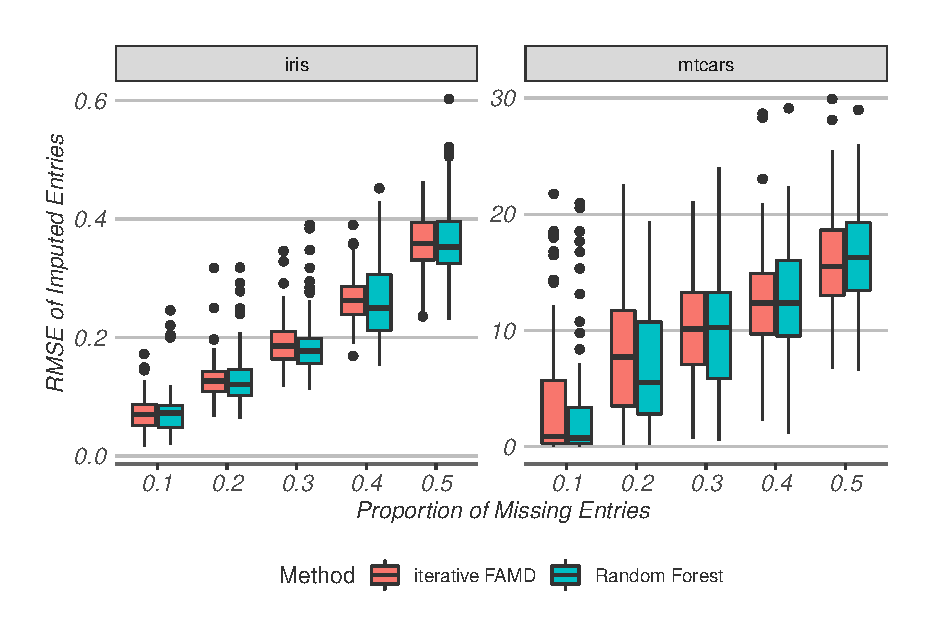
\includegraphics[width=0.9\textwidth]{./figures/rmse_mixed_dataset.eps}
        \caption{Distribution of the RMSE of Imputed Entries}
        \label{figure:rmse_mixed_dataset}
    \end{figure}

    \begin{figure}[!hbt]
        \centering
        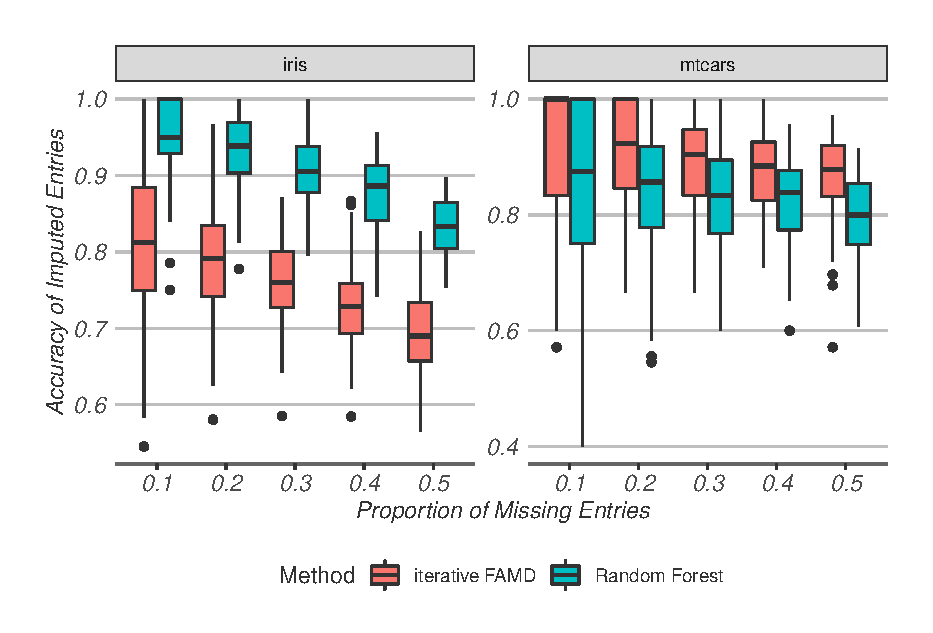
\includegraphics[width=0.9\textwidth]{./figures/accuracy_mixed_dataset.eps}
        \caption{Distribution of the Accuracy of Imputed Entries}
        \label{figure:accuracy_mixed_dataset}
    \end{figure}

    Our experiments seem not as good as described in the paper compared to the Random Forest method. In the Iris and mtcars datasets, the MSE estimated by the two methods of continuous data are relatively close, but the Random Forest is slightly better than the iterative FAMD approach. The accuracy of imputed values for the iterative FAMD is significantly better than the Random Forest approach in categorical data. Therefore, in the subsequent research, we need to spend more time exploring why our experimental results do not have the same performance in continuous and categorical data and exploring the structure of the data applicable to this method.

    \subsection{Prediction with Imcomplete Dataset}

    As we mentioned in the introduction, an actual application of matrix completion is that we can directly apply various statistical methods to the filled data set. Therefore, we use the dataset titanic in the Kaggle entry competition \citep{kaggle_titanic_2015} to illustrate this imputation method's influence in this respect.

    We continue to work based on \citet{hilla_titanic_2017}'s work, which constructed features such as title, family boating or not, and deleted more than 90\% missingness variable -- Cabin. After the above processing, the data missing is as follows (Table \ref{table:tianic_variables}). Our goal is to fill in the missing values so that standard statistical methods, such as logistic regression, can be used to predict the target variable.

    \begin{table}[!hbt]
        \centering
        \caption{Types of Variables and Missing Situations}
        \label{table:tianic_variables}
        \begin{tabular}{@{}ccc@{}}
        \toprule
        Variable & Data Type   & Missingness \\ \midrule
        Age      & Continuous  & 263/1309    \\
        Fare     & Continuous  & 1/1309      \\
        Embarked & Categorical & 2/1309      \\ \bottomrule
        \end{tabular}
    \end{table}

    To facilitate the evaluation of the iterative FAMD method's practicability, we use mean imputation, random forest, and the iterative FAMD method to fill in missing values. After the matrix is completed, we use logistic regression to predict the target variable.

    \begin{equation*}
        h_{\theta}(X)=\frac{1}{1+e^{-\theta^{T} X}}=\operatorname{Pr}(Y=1 \mid X ; \theta)
    \end{equation*}

    The results we get are as shown in Figure \ref{figure:titanic_roc} and Table \ref{table:titanic_metrics}. From the results, we can see no significant difference between the three filling methods under this data set. The iterative FAMD is slightly better than other methods, but we still need to see whether this method is still better than other methods in other situations...

    \begin{figure}[!hbt]
        \centering
        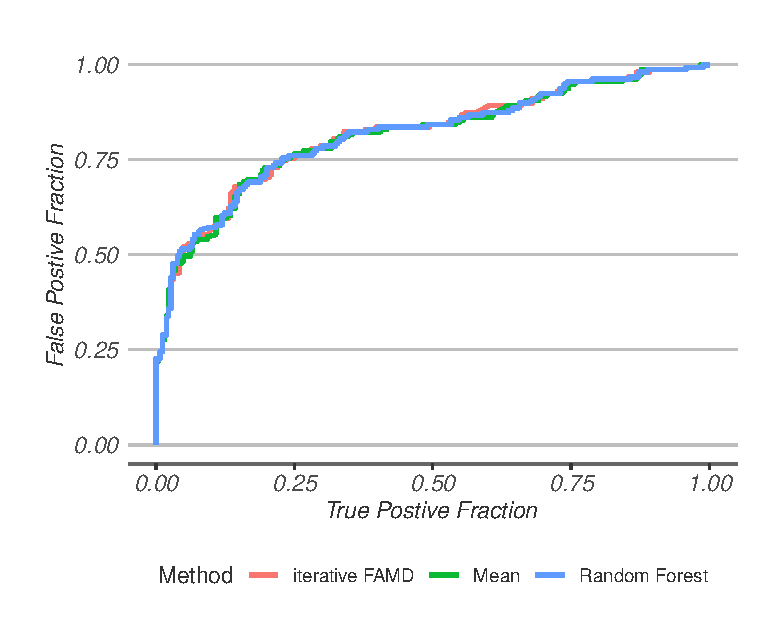
\includegraphics[width=0.65\textwidth]{./figures/titanic_roc.eps}
        \caption{ROC of Different Imputation Method with the Same Features and Model}
        \label{figure:titanic_roc}
    \end{figure}

    \begin{table}[!hbt]
        \centering
        \caption{Evaluation Metrics of Different Imputation Method with the Same Features and Model}
        \label{table:titanic_metrics}
        \begin{tabular}{@{}ccccc@{}}
        \toprule
                       & Accuracy & Precision & Recall & AUC    \\\midrule 
        Mean           & 0.7799   & 0.8571    & 0.8014 & 0.7556 \\
        Random Forest  & 0.7799   & 0.8533    & 0.8036 & 0.7568 \\
        iterative FAMD & 0.7871   & 0.8610    & 0.8080 & 0.7638 \\\bottomrule
        \end{tabular}
    \end{table}

    % \section{Proportion of Observations}

    % For \textit{Optimal adaptive matrix completion} \citep{ramazanli_optimal_2020}.

    \section{Missing Mechanism}

    Unfortunately, the approaches we mentioned before have focused on the similarities between individuals and the relationships between variables rather than the missing data's missing mechanism. \cite{little_statistical_2019} produced an early contribution to the missing mechanism, in which there were three typical assumptions in missing mechanism:
    \begin{itemize}
        \item MCAR, missing completely at random, the missingness does not depend on the values of the data, whether missing or observed. 
        \item MAR, missing at random, the missingness depends on $Y_{i,j}$ only through other covariates.
        \item MNAR, missing not at random, the missingness depends on $Y_{i,j}$ only through the unobserved value $Y_{i,j}$ itself.
    \end{itemize}
    Whether mentioned or not, the above methods are all based on assumptions MCAR with the same missing probability in the entire matrix, which are too strict and not close to the real world. Here, we further relax the assumptions. Moreover, it is a norm that the missingness mechanism is heterogeneous, as known as the missing probability are varies in a matrix across columns. For instance, some products may have more ratings in those columns since they are more popular than others. To use this information, we need to distinguish the missing data's probability in matrix completion.

    \subsection{The primePCA algorithm}

    For \textit{High-dimensional principal component analysis with heterogeneous missingness} \citep{zhu_high-dimensional_2019}, it converts the question in Equation \ref{equation:standard_matrix_completion} into the following form.
    \begin{equation}
        \bf{Y}=\bf{X}+\bf{Z}
    \end{equation}
    where $\bf Y\in\mathbb{R}^{n\times d}$ is the observed matrix, $\bf X\in\mathbb{R}^{n\times d}$ is the real matrix with a low rank assumption, $\bf Z\in\mathbb{R}^{n\times d}$ is a noise matrix with i.i.d normal gussian distribution.

    With the low rank assumption of $\bf X$, we can assume that it is generated via
    \begin{equation}
        \mathbf{X}=\mathbf{U} \mathbf{V}_{K}^{\top}
    \end{equation}
    where $\mathbf{V}_{K}\in\mathbb{R}^{d\times K}$ has orthonormal columns and $\mathbf{U}\in\mathbb{R}^{n\times K}$ is a random matrix having i.i.d distribution in rows with zero mean.

    In this paper, the focus is typically on the accurate recovery of the missing entries, subject to a low-rank assumption on the signal matrix; by contrast, their focus is on estimating the principal eigenspaces $\operatorname{Col}\left(\mathbf{V}_{K}\right)$.

    In order to solve this problem, they introduce a new method for high-dimensional PCA, called \textbf{primePCA} (as showm in Algorithm \ref{algorithm:primePCA}), that is designed to cope with situations where observations may be missing in a heterogeneous manner, which iteratively projects the observed entries of the data matrix onto the column space of our current estimate to impute the missing entries and then updates our estimate by computing the leading right singular space of the imputed data matrix.

    \begin{algorithm}[H]
        \KwData{$\hat{\bf V_{K}}^{(\mathrm{in})} \in \mathbb{O}^{d \times K}$, $K \in [d]$}
        \KwResult{$\hat{\bf V_{K}}^{(\mathrm{out})}$}
        \ForAll{$i$ in $[n]$}{
            $\mathcal{J}_i \leftarrow \{j \in [d]: \omega_{ij} = 1\}$\;
            $\hat {\bf u}_i \leftarrow (\hat{\bf V}_{K}^{(\mathrm{in})})_{\mathcal{J}_i}^{\dagger} \tilde{\bf y}_{i, \mathcal{J}_i}$\;
            $\hat{\bf y}_{i, \mathcal{J}_i^{\mathrm{c}}} \leftarrow \hat{\bf V}_{K}^{(\mathrm{in})} \hat{\bf u}_{i, \mathcal{J}_i^{\mathrm{c}}}$\;
            $\hat{\bf y}_{i, \mathcal{J}_i} \leftarrow \hat{\bf y}_{i, \mathcal{J}_i}$\;
        }
        $\hat{\bf Y} \leftarrow (\hat{\bf y}_{1}, \ldots, \hat{\bf y}_{n})^{\top}$\;
        $\hat{\bf V_{K}}^{(\mathrm{out})}\leftarrow$ top $K$ right singular vectors of $\hat{\bf Y}$\;
        \caption{\textbf{refine}, a single step of refinement of current iterate $\hat{\bf V_{K}}^{(\mathrm{in})}$ \citep{zhu_high-dimensional_2019}}
        \label{algorithm:refine}
    \end{algorithm}
    \begin{itemize}
        \item $\bf W$ is the matrix of weights such that $w_{i,j}=\left\{\begin{array}{ll}
            1 & (i, j) \in \Omega \\
            0 & \text { otherwise }
            \end{array}\right.$.
    \end{itemize}
    
    \begin{algorithm}[H]
        \KwData{$\hat{\bf V_{K}}^{(0)} \in \mathbb{O}^{d \times K}$, $K \in [d]$, $\sigma_* \in (0,\infty)$, $\kappa^* \in [0, \infty)$}
        \KwResult{$\hat{\bf V_{K}}$}
        \For{$i$ in $[n]$}{
            $\mathcal{J}_i \leftarrow \{j \in [d]: \omega_{ij} = 1\}$\;
        }
        \While{$L(\hat{\bf V}^{(t)}_{K}, \hat{\bf V}^{(t - 1)}_{K}) < \kappa^*$}{
            $\mathcal{I}^{(t-1)} \leftarrow \{i: \|\bf\omega_i\| > K, \sigma_{K}( (\hat{\bf V}_{K}^{(t-1)})_{\mathcal{I}}) \geq \frac{|\mathcal{I}|^{1/2}}{d^{1 / 2}\sigma_*}\}$\;
            \tcc{Define in Algorithm \ref{algorithm:refine}}
            $\hat{\bf V_{K}}^{(\mathrm{t})} \leftarrow \operatorname{refine}\left(\hat{\bf V_{K}}^{(\mathrm{t-1})}, K\right)$\;
        }
        $\hat{\bf V}_{K}\leftarrow\hat{\bf V}^{(t)}_{K}$\;
        \caption{\textbf{primePCA}, an iterative algorithm for estimating $\bf{V}_K$ given initialiser $\hat{\bf V_{K}}^{(0)}$ \citep{zhu_high-dimensional_2019}}
        \label{algorithm:primePCA}
    \end{algorithm}
    \begin{itemize}
        \item The initialization $\hat{\bf V_{K}}^{(0)}$ is the matrix of top $K$ eigenvectors of
        \begin{equation*}
            \tilde{\mathbf{G}}:=\frac{1}{n} \sum_{i=1}^{n} \tilde{\mathbf{y}}_{i} \tilde{\mathbf{y}}_{i}^{\top} \circ \tilde{\mathbf{W}}
        \end{equation*}
        where $\tilde{\mathbf{W}}_{j k}:=\left\{\begin{array}{ll}\frac{n}{\sum_{i=1}^{n} \omega_{i j} \omega_{i k}} & \text { if } \sum_{i=1}^{n} \omega_{i j} \omega_{i k}>0 \\ 0, & \text { otherwise }\end{array}\right.$.
    \end{itemize}

    \subsection{Comparison on the Real Dataset}

    The example of commodity purchase record mentioned at the beginning is a widespread recommendation system problem, which can also be solved by the primePCA method. (Unfortunately, the filling method mentioned earlier in this article cannot be used to solve this problem because the missing ratio of the matrix is too large.) Here, we use the \textbf{MovieLens100k} data set to verify the primePCA algorithm and compare it with the softImpute and the Collaborative Filtering methods.

    \begin{quotation}
        \noindent
        \textbf{MovieLens100k} was collected through \href{https://movielens.org/}{the MovieLens web site} during the seven months from September 19th,  1997 through April 22nd, 1998. This data has been cleaned up - users who had less than 20 ratings or did not have complete demographic information were removed from this data set. The data set consists of 100,000 ratings (e.g., ratings of 1 through 5 stars) of 1,682 movies by 943 people.
    \end{quotation}

    The methods we compared are as follows:
    \begin{itemize}
        \item \textbf{UBCF}: User-based CF is a memory-based algorithm that tries to mimics word-of-mouth by analyzing rating data from many individuals. The assumption is that users with similar preferences will rate items similarly. Thus, missing ratings for a user can be predicted by first finding a neighborhood of similar users and then aggregating these users' ratings to form a prediction. \citep{hahsler_recommenderlab_2020}
        \item \textbf{IBCF}: Item-based CF is a model-based approach which produces recommendations based on the relationship between items inferred from the rating matrix. The assumption behind this approach is that users will prefer items that are similar to other items they like. The model-building step consists of calculating a similarity matrix containing all item-to-item similarities using a given similarity measure. \citep{hahsler_recommenderlab_2020}
        \item \textbf{softImpute}: Iterative methods for matrix completion that use nuclear-norm regularization. There are two main approaches.The one approach uses iterative soft-thresholded svds to impute the missing values. The second approach uses alternating least squares. \citep{mazumder_softimpute_2015}
        \item \textbf{primePCA}: After we get eigenspaces by Algorithm \ref{algorithm:primePCA}, we follow Algorithm \ref{algorithm:refine}'s step 2 to step 5 to get the recovered matrix.
    \end{itemize}

    To evaluate the model more effectively, we may ignore users that have provided too few ratings and also ignore those movies that have received too few ratings from users. Here we restrict the model training to those users who have rated at least 50 movies and those movies that have been rated by at least 100 users. This improves the proportion of non-missing entries.

    In order to make an objective comparison, we use the calculation method mentioned by \citet{hahsler_recommenderlab_2020}. For the Mean Average Error (MAE)
    \begin{equation*}
        \mathrm{MAE}=\frac{1}{|\mathcal{K}|} \sum_{(i, j) \in \mathcal{K}}\left|r_{i j}-\hat{r}_{i j}\right|
    \end{equation*}
    where $\mathcal{K}$ is the set of all user-item pairings $(i, j)$ for which we have a predicted rating $\hat{r}_{i j}$ and a known rating $r_{i j}$ which was not used to learn the matrix completion model. Furthermore, it is the same for the Root Mean Square Error (RMSE). The estimation results are shown in the Figure \ref{figure:ml10m}.

    \begin{figure}[!hbt]
        \centering
        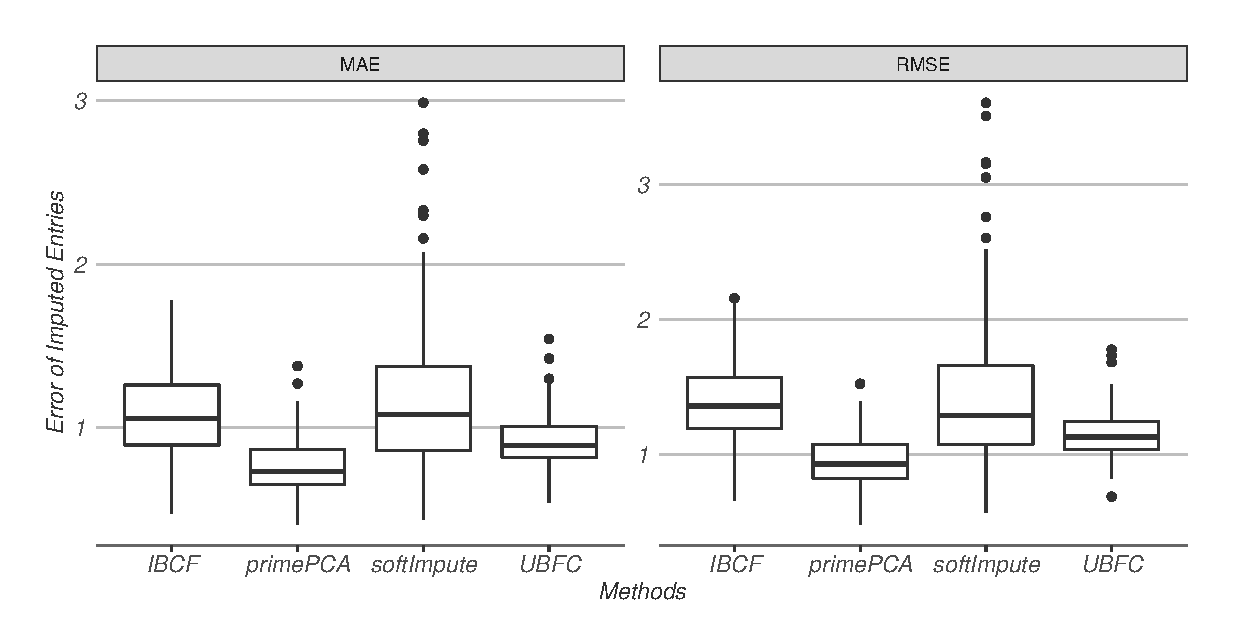
\includegraphics[width=0.9\textwidth]{./figures/ml10m.eps}
        \caption{Error of Imputed Entries by Users in IBCF, UBCF, softImpute and primePCA approaches}
        \label{figure:ml10m}
    \end{figure}

    The primePCA has obvious advantages over the other three methods. It has lower bias and variance, and this is because the method takes into account the heterogeneity in the estimation, which brings a lot of inspiration for our subsequent research on the matrix completion problem.\footnote{All of the experiment code are available at \href{https://github.com/signorinoy/sentry/}{https://github.com/signorinoy/sentry/}.}
    
    \clearpage
    \bibliography{ref}
\end{document}